\chapter{应用语义关系自动构建情感词典}
\label{ch2}
%本章将进入论文排版的正文, 按元素分主要包括:
%{\kai 字体段落,图片表格,公式定理,参考文献}这几部分。
%这个样例文件将包括模板中使用到的所有格式、模板中自定义命令到或者特有的东西,
%都将被一一介绍,希望大家在排版自己的学位论文前能细致的看一遍,记住样例的格式和
%方法,方便上手。

\section{引言}
\label{ch2:intro}
上一章主要介绍了本文的研究背景,要研究的科学问题,研究内容与方法,并指出观点分析研究一项基础的工作就是研究如何针对不同应用构建具有足够覆盖面并且良好适应性的情感知识词典。人在使用语言表达情感或观点时,最基本的方式是使用具有明确情感色彩的词汇,因此为了分析用户的观点,最直接的方法应该从用户产生文本中使用的词语开始,将语言中经常使用的词语所表达的情感信息进行汇总形成的词典就是情感词典。观点分析研究首先是在英文文本上开始的,情感词典相关研究也是从英文为主,方法相对比较成熟,形成了一些经常使用的英文情感词典资源。中文情感分析研究起步较晚,缺乏普遍认可的可靠的中文情感词典\upcite{朱嫣岚2006,朱征宇2013,黄硕2013}。目前研究使用主要有HowNet情感词典\upcite{2013},NTUSD情感词典\upcite{Ku2007}以及大连理工大学的情感词汇本体词库\upcite{2013a}。这些词典主要是以手工或半自动方式编辑而成,覆盖度、可靠性和领域适应性受到限制,并且情感词以主要积极和消极二值区分,缺少情感极性值的细粒度划分。能够将资源丰富的英文词典中的情感知识跨语言向中文词典进行适应性的转化,构建相应的中文情感词典资源,既可以省去耗费大量人力的人工标注过程,又可以克服目前中文情感词典自动或半自动构建方法的可靠性和覆盖度问题。
因此本章提出将英文情感词典资源情感知识转化为中文情感词典的构建方法,可以根据语义关系将英文词语及其情感极性值转化得到中文词语的情感极性值,并且完全是自动的,可靠性更高。下一章将该方法构建的情感词典在领域语料中进行扩展,以提高其领域覆盖度和适应性。

本章具体安排如下:首先对情感词典构建需要考虑的问题以及相关工作进行全面的介绍,接着对本章要使用的词典资源进行介绍,然后详细阐述如何利用一个双语语义知识库将英文情感词典情感知识转化为中文情感词典相应的词语情感信息,最后对该方法进行实验验证和说明。

\section{相关工作}
构建情感词典需要考虑词典覆盖面(Coverage)、词典内容(Content)以及构建方法(Acquisition)三个方面问题,具体内容可以用图~\ref{fig2-1-1}框架来展示。

\begin{figure}[htp]
\centering
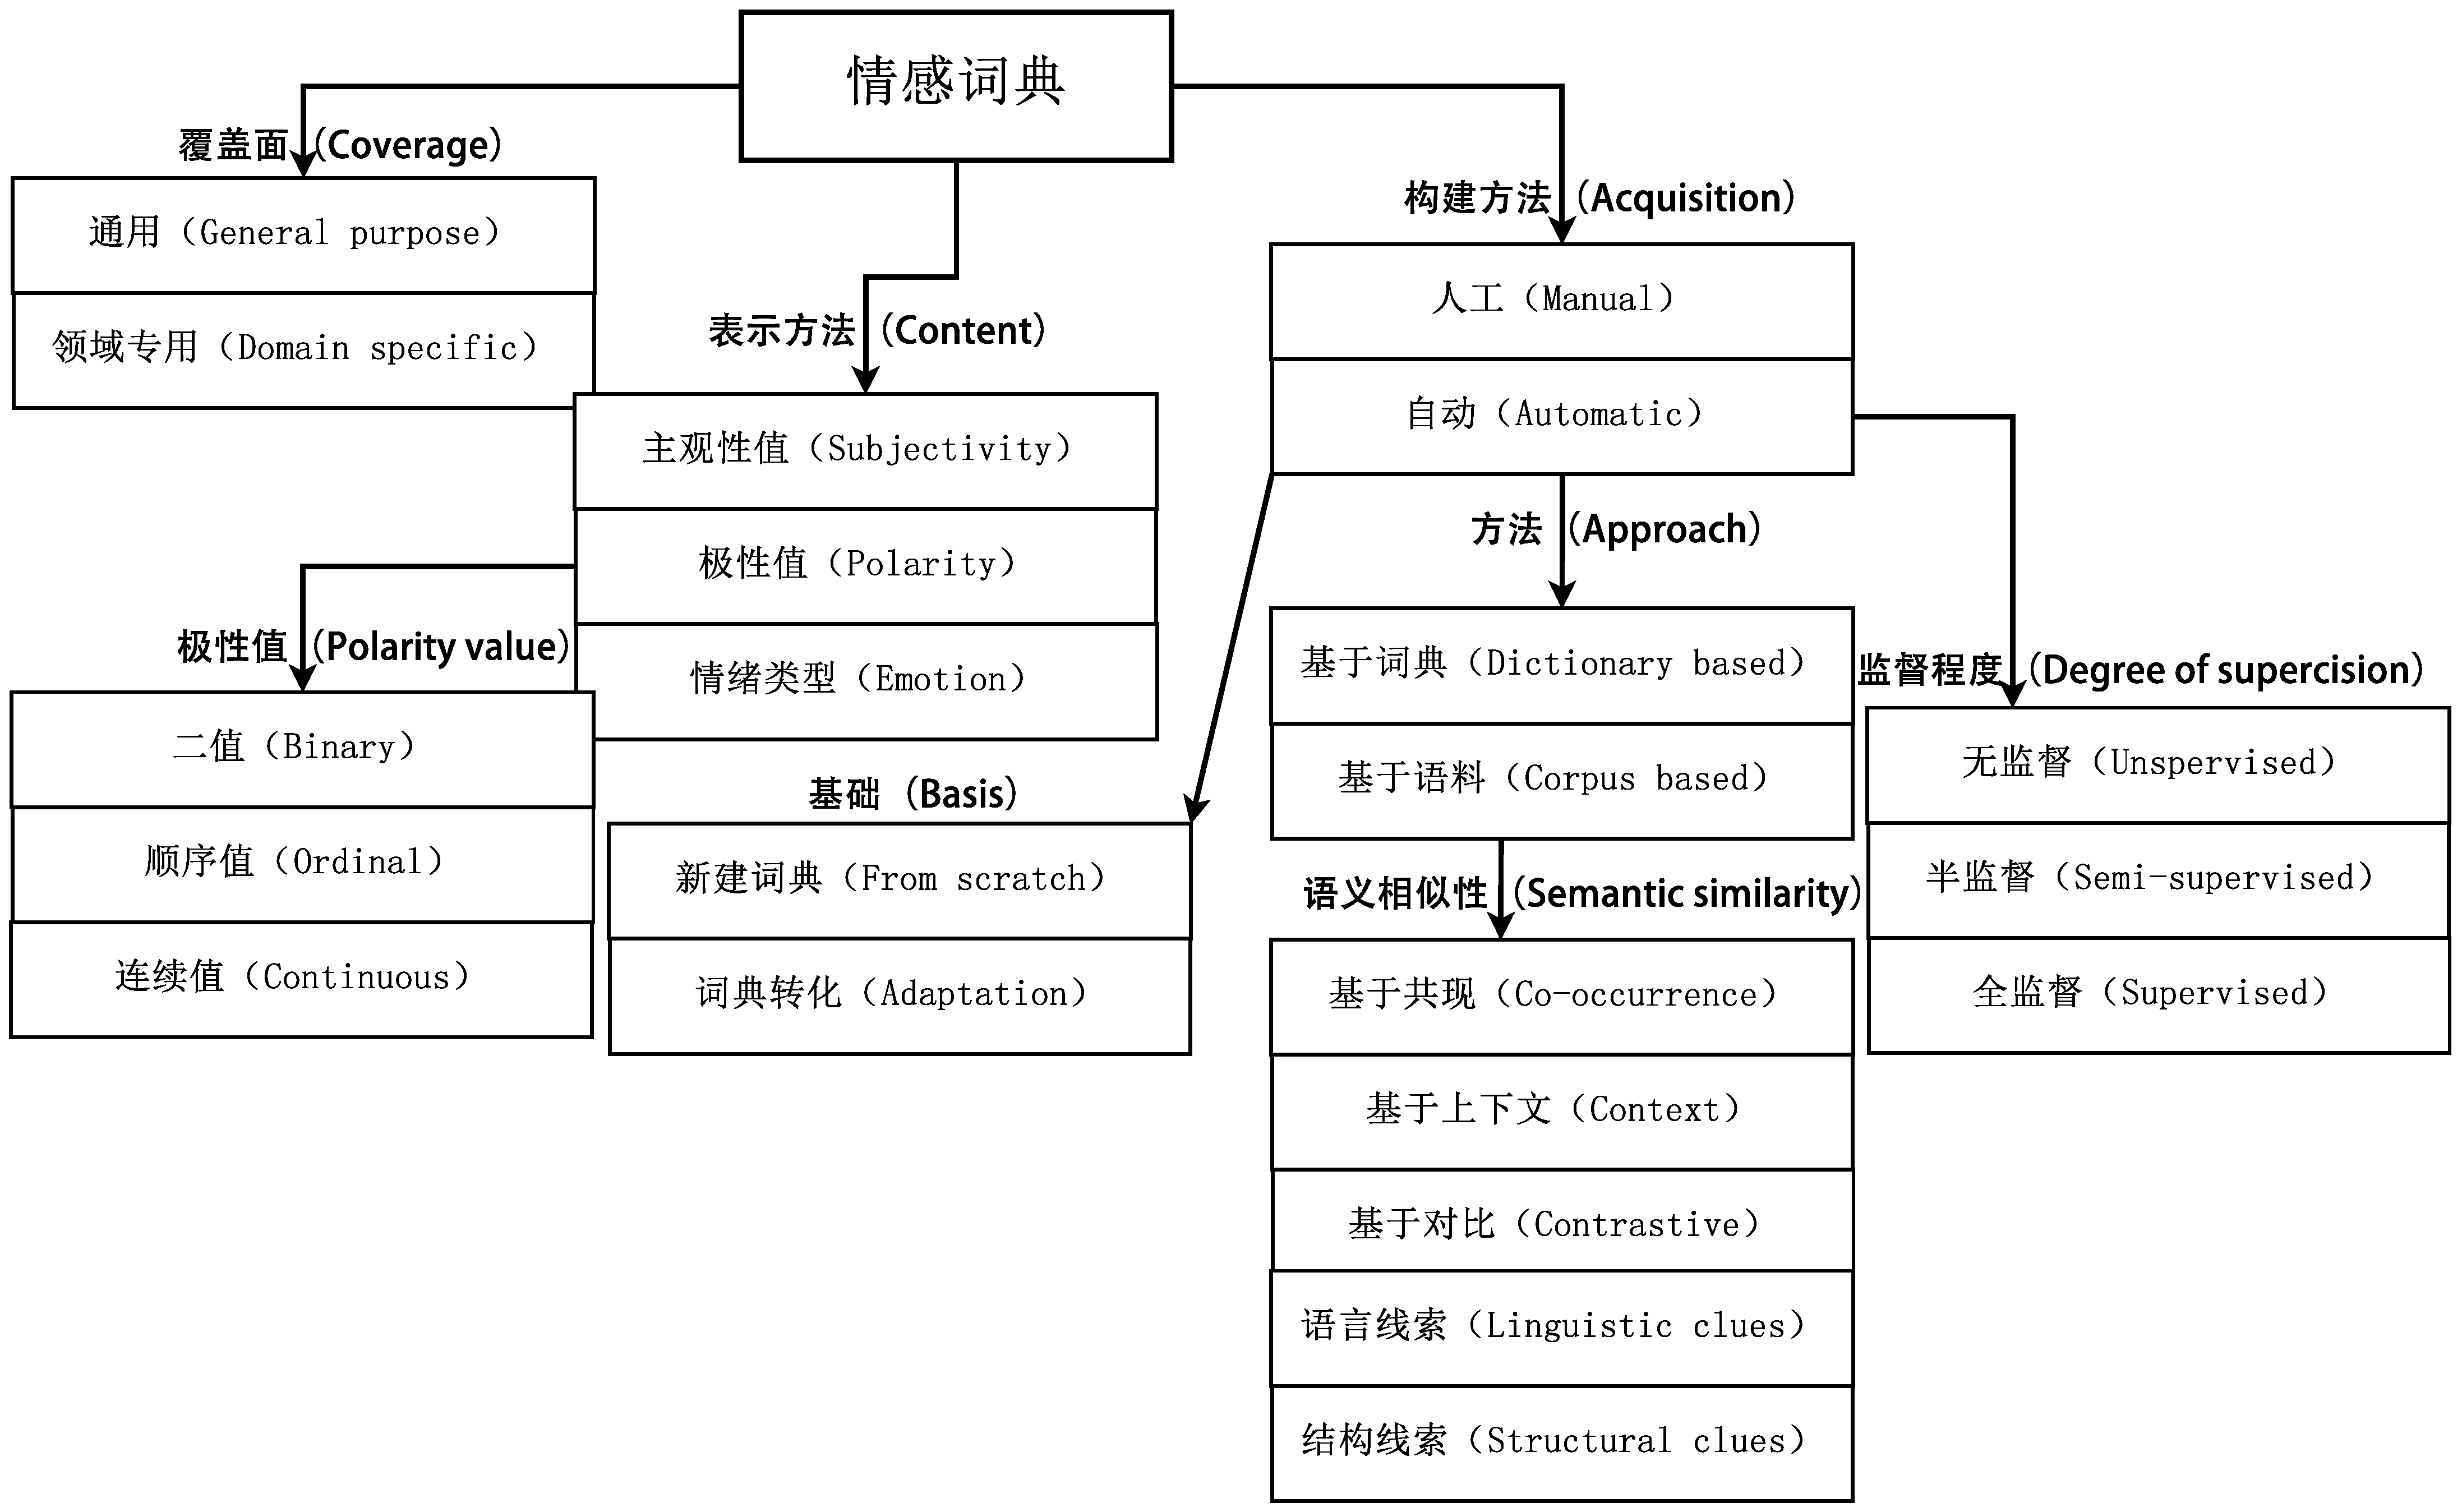
\includegraphics[height=300pt]{2-1-1.eps}
\caption{情感词典有关内容}
\label{fig2-1-1}
\end{figure}

\subsection{词典覆盖面}
就词典的覆盖面来讲,情感词典可以分为通用的词典以及领域专用的词典。构建通用情感词典的主要假设就是希望词语表达的情感独立于具体的领域和应用,这对一部分词语(比如:“赞”、“爱”、“憎恨”等),目前经常使用的情感词典基本都是通用的情感词典。但是实际上很多词语表达的情感是依赖于领域和具体的语境的,比如“轻薄”一词,一般情况表示负面情感,但是描述手机时却可以表示正面的评价。而且,一些本身不表示具体情感的词语(比如:“长”、“短”、“老”、“经典”等),用到一些特殊的语境时也会表达出一些具体情感(比如:“手机待机时间长”与“手机待机时间短”)。最近开始有一些研究开始针对具体领域和应用需求构建一些领域专用的情感词典\upcite{Choi2009,Du2010,Klenner2009}。

\subsection{词典内容}
情感词典可以就其表示情感知识内容进行细分,当然情感知识表示方法与具体的应用场景是密切相关的,我们不考虑具体的应用场景,而仅仅对词典的情感表示方法进行划分。从这个方面来看,情感词典表示情感知识的方法可以分为三种:词语表示主观性的程度(Degree of subjectivity)、表示情感的极性(Polarity)或者表示的情绪类型(Emotion\/mood,比如喜、怒、哀、乐等)。表示主观性程度的情感词典主要用于文本主观性的探测任务\upcite{CarmenBanea2008,Gyamfi2009,Maks2012,Wiebe2000,Wiebe2006},而主观文本表达观点的具体情感类型的识别,需要表示情感极性或情绪类型的情感词典。在情感分类中经常使用是表示情感极性的词典,其中的词语都标注了表达的情感极性是积极的还是消极的,这对于想要确定文本所表达观点的倾向性是非常重要的。对这类情感词典还可以根据表示的情感极性值大小进一步划分:比如使用二值情感极性(也就是积极的和消极的)的情感词典\upcite{Godbole2007,Hatzivassiloglou1997,Hu2004,Rao2009};使用顺序值(ordinal)表示极性值的情感词典,比如常使用1-5整数值区分情感极性的强度值\upcite{Yessenalina2011};还有一些使用连续数值(continuous)表示情感极性强度的情感词典\upcite{Turney2003,Sasha2008,Velikovich2010,Remus2010}。
目前有很多这样的英文情感词典,比如:OpinionFinder(OF)\upcite{Wilson2005d},Appraisal Lexicon(AL)\upcite{Taboada2004},SentimentWordNet\upcite{Baccianella2010}以及Q-WordNet\upcite{Agerri2010}等。

如果为了分析更细粒度(fine-grained)的情感,需要将词语表达的情感根据情绪类型进行表示,比如Bollen等\upcite{bollen2011twitter}通过分析Twitter中大众表达出的不同情绪来预测股票指数的变化,Garcia和Schweitzer\upcite{Garcia2011}对产品评论中的情绪类型进行了细致研究,类似的工作还有Davidov等\upcite{Davidov2010}以及Strapparava和Mihalcea\upcite{Strapparava2008}在Twitter上的工作。这种类型的情感词典都是靠人工编辑形成的,比如GI(General Inquirer)\footnote{\url{http://www.wjh.harvard.edu/~inquirer/Home.html}}\upcite{Stone1966},ANEW(Affective Norms for English Words)upcite{Bradley1999},WordNet-Affect\footnote{\url{http://wndomains.fbk.eu/wnaffect.html}}upcite{Valitutti2004,Valitutti2004a},DAL (Dictionary of Affect in Language)upcite{Whissell1989}等词典。

\subsection{词典构建方法}
从情感词典的构建方法来看,可以分为人工构建和自动构建两种类型。目前公开可用的人工编辑的情感词典基本都是通用的情感词典(比如:OF词典和GI词典),人工构建情感词典主要面临的问题除了需要耗费大量的人力,还有覆盖面相对较低,以及需要对不同的领域进行适应性扩展才能达到好的观点分析效果。

而对于自动构建情感词典方法,还可以按照方法(Approach)、监督程度(Degree of supervision)和构建基础(Basis)三个维度进行区分。

\subsubsection{构建方法}
情感词典主要的构建方法分为两类:一是基于词典(dictionary-based)方法,根据已有词典的词语之间的语义关系判断词语的情感极性或计算情感极性值;二是基于语料(corpus-based)方法,根据词语在语料中的分布特点推导出情感极性并计算极性值。两类方法共同特点是都需要一个预先标注的种子词集(seed set),然后通过不断迭代计算词语与种子词集词语之间的某种语义相似性,推导词语情感极性值并扩充种子词集,直到收敛。

\paragraph{基于词典方法:}
基于词典的方法通常会使用一个词库(thesaurus)或语义知识库(比如常用的是WordNet\upcite{Miller1995}),并且常用的假设是词语间的语义关系转换词语的情感信息,最常用的语义关系是词语间的同义和反义关系\upcite{Godbole2007,Kim2006,Ahsaee2010}。例如形容词“lovely”会将积极极性通过同义关系传递给“admirable”、“adorable"”、“amiable”和“pretty”,反过来会将消极极性转换给反义词语“awful”、“unlovely”和“ugly”。但是这种转换会随着语义距离增加而弱化,比如在WordNet中从“good”到“bad”的同义关系距离长度只有3\upcite{Godbole2007},因此方法设计时需要采取适当措施将语义距离考虑在内\upcite{Godbole2007,Ide2006,Budanitsky2001,Kim2006,Ahsaee2010}。除了同义和反义关系,一些研究提出使用WordNet中的其他语义关系,比如“similarity”,“derived-from”,“pertains-to”,“also-see”或“attribute”等关系\upcite{Esuli2006,Valitutti2004a}。Takamura等\upcite{Takamura2005}以及Andreevskaia等\upcite{Andreevskaia2006}使用了并不直观的下位关系(hyponymy)构建情感词典。还有一些方法通过计算词语在词典中解释的相似性来度量词语间的语义相关性,然后根据这种语义相关性构建情感词典\upcite{Esuli2006,Baccianella2010,Takamura2007}。

\paragraph{基于语料方法:}
和基于词典方法一样,基于语料方法一个基本思想就是通过某种方法度量词语间的语义相关性,然后从标注好的种子集中推断出词语的情感信息。这些度量方法可以分为以下四种:
\begin{itemize}
\item \textbf{基于词语共现方法}:代表性的工作是Turney等\upcite{Turney2002,Turney2003},主要是假设“一个词语的语义倾向性(semantic orientation)\footnote{Turney使用语义倾向性指代词语的情感极性}往往与其相邻的词语的语义倾向性相关”,因此他们使用点互信息(pointwise mutual information)PMI统计对词语和种子词集的相关性进行度量,推导出词语的情感极性。
\item \textbf{基于上下文方法}:除了直接通过共现来度量两个词语的相关性,在统计语义学还有还有一种常用的方法就是使用词语的上下文信息。在Firth的《Contextual Theory of Meaning》一书中,提出一个基本的假设就是“a word is characterized by the company it keeps”\upcite{Firth1957},因此词语的语义信息是与上下文语境紧密相关的。因此一些基于语料的情感词典构建方法利用这一假设,提出在相似上下文出现的词语很有可能具有相似的情感信息,因此可以从情感极性已知的种子词集推导出其他词语的情感极性\upcite{Baron2003,Wiebe2000,Velikovich2010}。
\item \textbf{基于对比方法}:该类方法将前台(foreground)语料和背景(background)语料对比分析进行情感词语的抽取构建情感词典。比如Maks和Vossen\upcite{Maks2012}研究了对数似然和相对频率比提取主观词构建语情感词典,他们使用报纸新闻以及新闻评论作为主观前台语料,维基百科文本作为客观背景语料。相似的工作还有Stepinski和Mittal\upcite{Stepinski2007}。
\item \textbf{基于语言线索}:前面几种方法单纯依靠语料中统计出的信息,不考虑对文本的深层次语言学分析。其实已经有工作确认一些常用的语言模式有助于词语的情感信息的探测。Hatzivassiloglou和McKeown\upcite{Hatzivassiloglou1997}发现一个句子中连词(“and”和“but”)对与所连接的两个词语的情感极性具有一定的限制作用,出现在“and”两边的词语一般具有相同的极性,而出现在“but”两边的词语极一般性相反,他们利用这种限制从文本语料中抽取并构建情感词典。在产品评论的观点挖掘研究中一些工作扩展了这种连词语言线索,同时考虑了跨句子的连词\upcite{Ding2008,Angel,Kanayama2006,Popescu2007}。
\item \textbf{基于结构线索}:代表性的工作是Kaji和Kitsuregawa\upcite{Kaji2006,Kaji2007}的工作,他们利用HTML文档中的结构线索分别抽取情感极性为积极和消极的句子集,从大量HTML文档中抽取出大概500,000主观句子用于训练情感分类器并构建情感词典。
\end{itemize}

\subsection{词典转化}
上述的所有情感词典构建方法都是从头开始(from scratch)构建新的情感词典,最近也有一些方法研究已有情感词典进行转化,主要是增强通用情感词典的领域适应性或者从单语言情感词典扩展到多语言。通用情感词典进行领域转化方法,主要有Choi和Cardie\upcite{Choi2009}提出的基于线性规划方法,Du等\upcite{Du2010}提出的基于信息理论框架以及Qiu等\upcite{Qiu2009}使用语言模式的扩展方法等。Mihalcea等\upcite{Mihalcea2007}提出了基于词典和基于语料的方法将英文情感词典通过翻译转化为其他语言的情感词典。

\subsection{混合方法}
混合方法指的是构建情感词典时将多种词典和语料资源结合起来。例如Hoang等\upcite{Hoang2008}提出使用WordNet的语义关系产生初始情感词典,然后使用从网络语料中获取的统计信息对其进行完善,词典资源和语料资源用一个错误最小化算法(error minimization algorithm)结合起来。Lu等\upcite{Lu2011}提出将四种信息组合起来确定词语的情感极性,包括从一个通用情感词典得到的信息,从一个词库(thesaurus)得到的信息,以及从一个领域文档集中得到的语言线索和结构线索信息,这四种信息通过一个基于线性规划的优化框架结合起来确定词语的情感极性。

综上所述,目前有很多种构建情感词典方法,以针对英文资源的构建方法研究为主。中文情感词典的构建方法研究还相对较少,而且基本上是借鉴英文的构建方法,而且形成的中文情感词典表示的情感知识是简单的二值极性。本章主要研究如何从英文词典进行转化得到中文情感词典,属于词典转化方法,但是我们的实现方法是借助于双语语义知识库中的语义关系实现这种转化,而不是使用翻译的方式,而且我们形成的情感词典能够通过计算将英文情感词典的情感极性值同时转化过来,情感知识更加丰富。

%随着互联网的发展,尤其是社交网络的发展,各种社交媒体的用户发布内容中出现了海量含有用户主观情感色彩的文本数据。针对网络文本的信息处理开始由获得关键词\upcite{Yuan2013}、事件
%\upcite{张辉2013}、话题\upcite{刘健2013} 等事实信息,开始向情感观点等主观信息深入,情感分析便是近年来迅速发展的信息处理技术\upcite{Liu2012}。从数据中提炼出用户的主观信息对于商业情报、舆情分析等具有重要意义。情感分析技术就是对带有情感色彩的主观性文本进行自动推理、分析、归纳的过程,涉及自然语言处理、机器学习、认知科学以及社会心理学等方面的研究\upcite{黄萱菁2011}。


\section{词典资源简介}
\label{ch2:lex}
本节简要介绍要用到的一些词典和知识库资源,主要是针对本章研究相关部分作介绍。
\subsection{HowNet语义知识库}
HowNet是一个以中英文词语所代表的概念为描述对象,揭示概念与概念之间以及概念的属性与属性之间的关系的知识库\upcite{杜飞龙2000}。HowNet两个重要名词是“义原”和“概念”:概念是对词汇语义的一种描述,每一个词可以表达为几个概念\upcite{刘群2002};义原是最小语义单元,用于定义和描述概念。
\subsubsection{义原} 
HowNet设计了大概2200多个义原,这些义原分为几个大类,具体参见表~\ref{tab2-1}。

\begin{table}[htp]
\centering
\caption{HowNet义原分类}
\label{tab2-1}
\begin{threeparttable}
 \begin{tabular}{|l|l|l|l|}
 \hline
 义原&数量& 示例&语义倾向性\tnote{1}\\
 \hline
 Event$ | $事件& 819& blame$ | $埋怨& 一般有倾向性\\
 \hline
Entity$ | $实体& 142& human$ | $人 & 不具倾向性\\
\hline
Attribute$ | $属性& 117 & length$ | $长度 &一般不具倾向性\\
\hline
aValue$ | $属性值& 899 & good$ | $好 &一般有倾向性\\
\hline
Quantity$ | $数量& 3 & rate$ | $比率 & 一般不具倾向性\\
\hline
qValue$ | $数量值& 13 & ufficient$ | $足 & 一般有倾向性\\
\hline
SecondaryFeature$ | $次要特征& 100 & desired$ | $良&一般有倾向性\\
\hline
Semanticroles$ | $语义角色& 90 & StateFin$ | $终状态 & 一般不具倾向性\tnote{2}\\
 \hline
\end{tabular}
\begin{tablenotes}
%  \centering
  \footnotesize
\item[1]语义倾向性即情感极性。
\item[2]虽然语义角色类不具有倾向性,但是代表的语义关系可以影响其他义原的倾向性。
\end{tablenotes}
\end{threeparttable}
\end{table}

表中可以看出,除了事物类、属性类以及数量类义原,其他义原一般都具有情感极性,并且义原都是由中英双语标识,因此可以通过英文标识从英文情感词典中获得其情感极性值。但是有一部分义原的英文标识不是一个单词(比如:FondOf$ | $喜欢,WhileAway$ | $消闲等),无法直接从英文情感词典直接获得情感极性值。实际上义原之间并不是独立的,义原之间存在复杂的关系,HowNet中描述了义原之间的主要的8种关系:上下位关系、同义关系、反义关系、对义关系、属性-宿主关系、部件-整体关系、材料-成品关系、事件-角色关系。义原之间组成的是一个复杂的网状结构,而不是一个简单树状结构。不过,义原关系中最重要关系是上下位关系,义原根据上下位关系形成了如图\ref{fig2-2}树状层次体系,我们可以借助其对无法直接转化得到情感值那部分义原的情感极性值的计算。

\begin{figure}[htp]
\centering
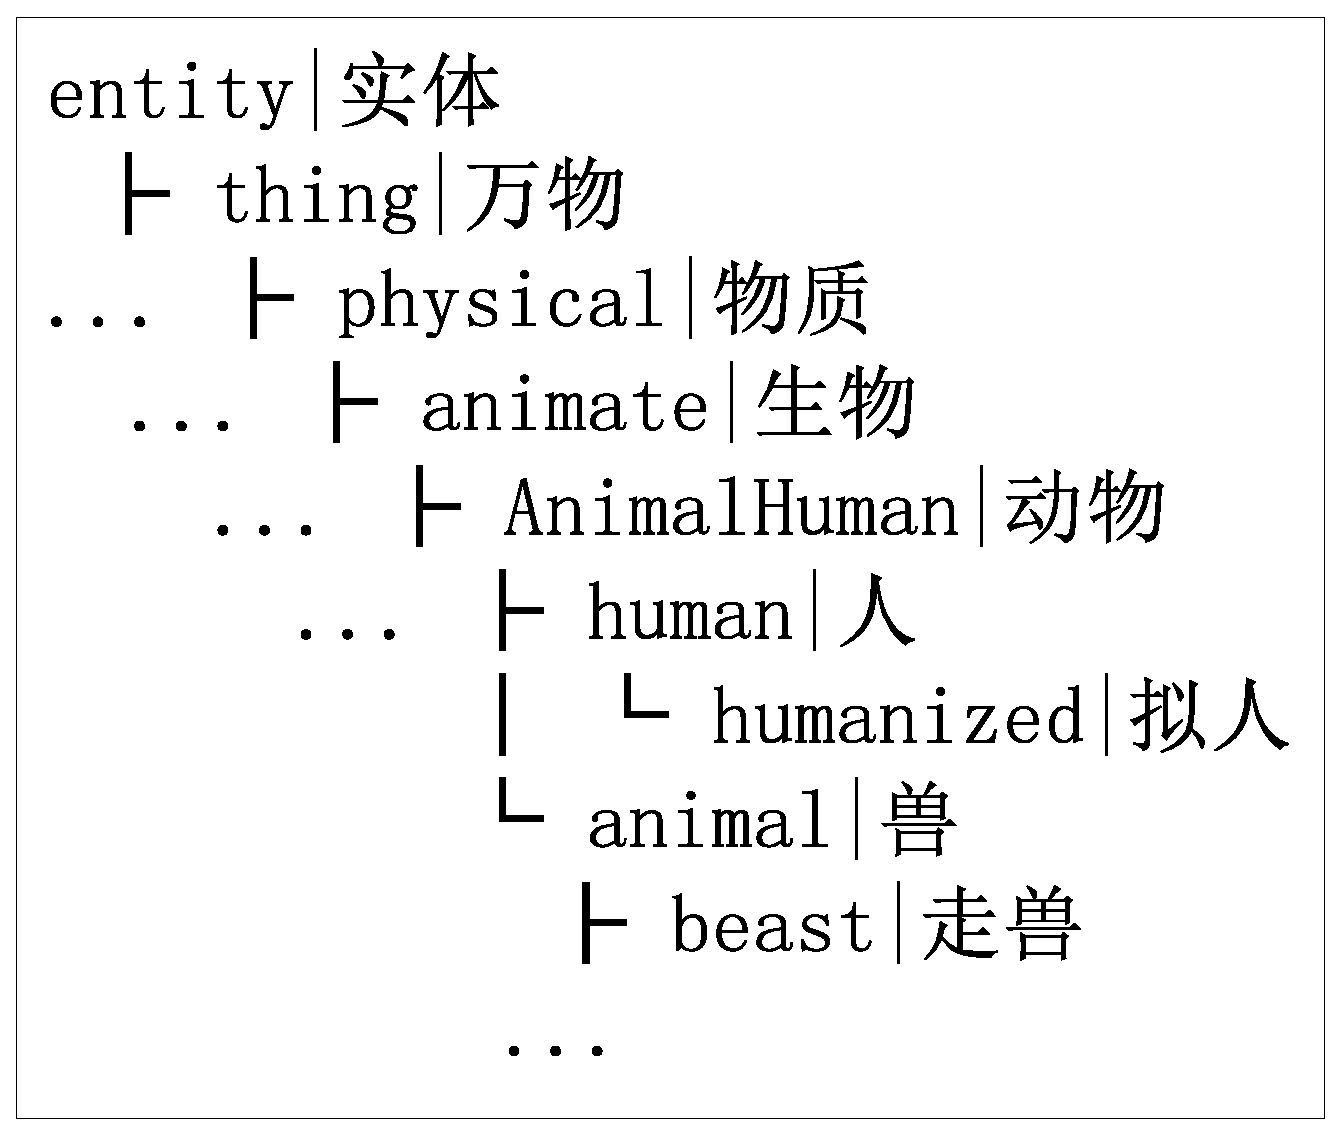
\includegraphics[height=170pt]{2-1-0.eps}
\caption{HowNet义原层次结构}
\label{fig2-2}
\end{figure}

除了义原以外,HowNet还有一些符号(或称为符号义原)对概念语义描述,可以把这些符号归为几类:第一类包括“$ , $”(表示“和”的关系)、“$\sim $”(表示“或”的关系)、“$ \wedge$”(表示“非”的关系),用来表示语义描述式之间的逻辑关系;第二类包括“$\#, \%, \$, \& ,\ast,+,?,!,@ $”,表示概念之间以及概念的属性之间的关系;第三类包括几个无法归入以上两类的特殊符号“$\{\}, \left( \right), \left[ \right]$” 。这些符号义原中第一类描述逻辑关系的三个符号会引起所描述义原情感极性的变化,尤其是“$ \wedge$”会引起情感极性的反转。

\subsubsection{概念}
如图~\ref{fig2-3}所示,HowNet采用KDML(Knowledge Dictionary Mark-up Language)语言描述概念,其中W\_X表示词语,G\_X表示词语词性,E\_X表示词语例子,X为C时表示中文,X为E时表示英文。
%DEF是对于该概念的定义项,称之为一个语义表达式,其中中英文标注的是义原,“\#\*”等标示符号来对概念属性之间关系进行描述,DEF中还可以包含概念,概念之间相互交织构成一个网。HowNet一共有2234个义原,收录了近15万条概念记录,涵盖了绝大部分中文常用词语,本章将基于HowNet的词语进行情感词典的构建。

\begin{figure}[htp]
\centering
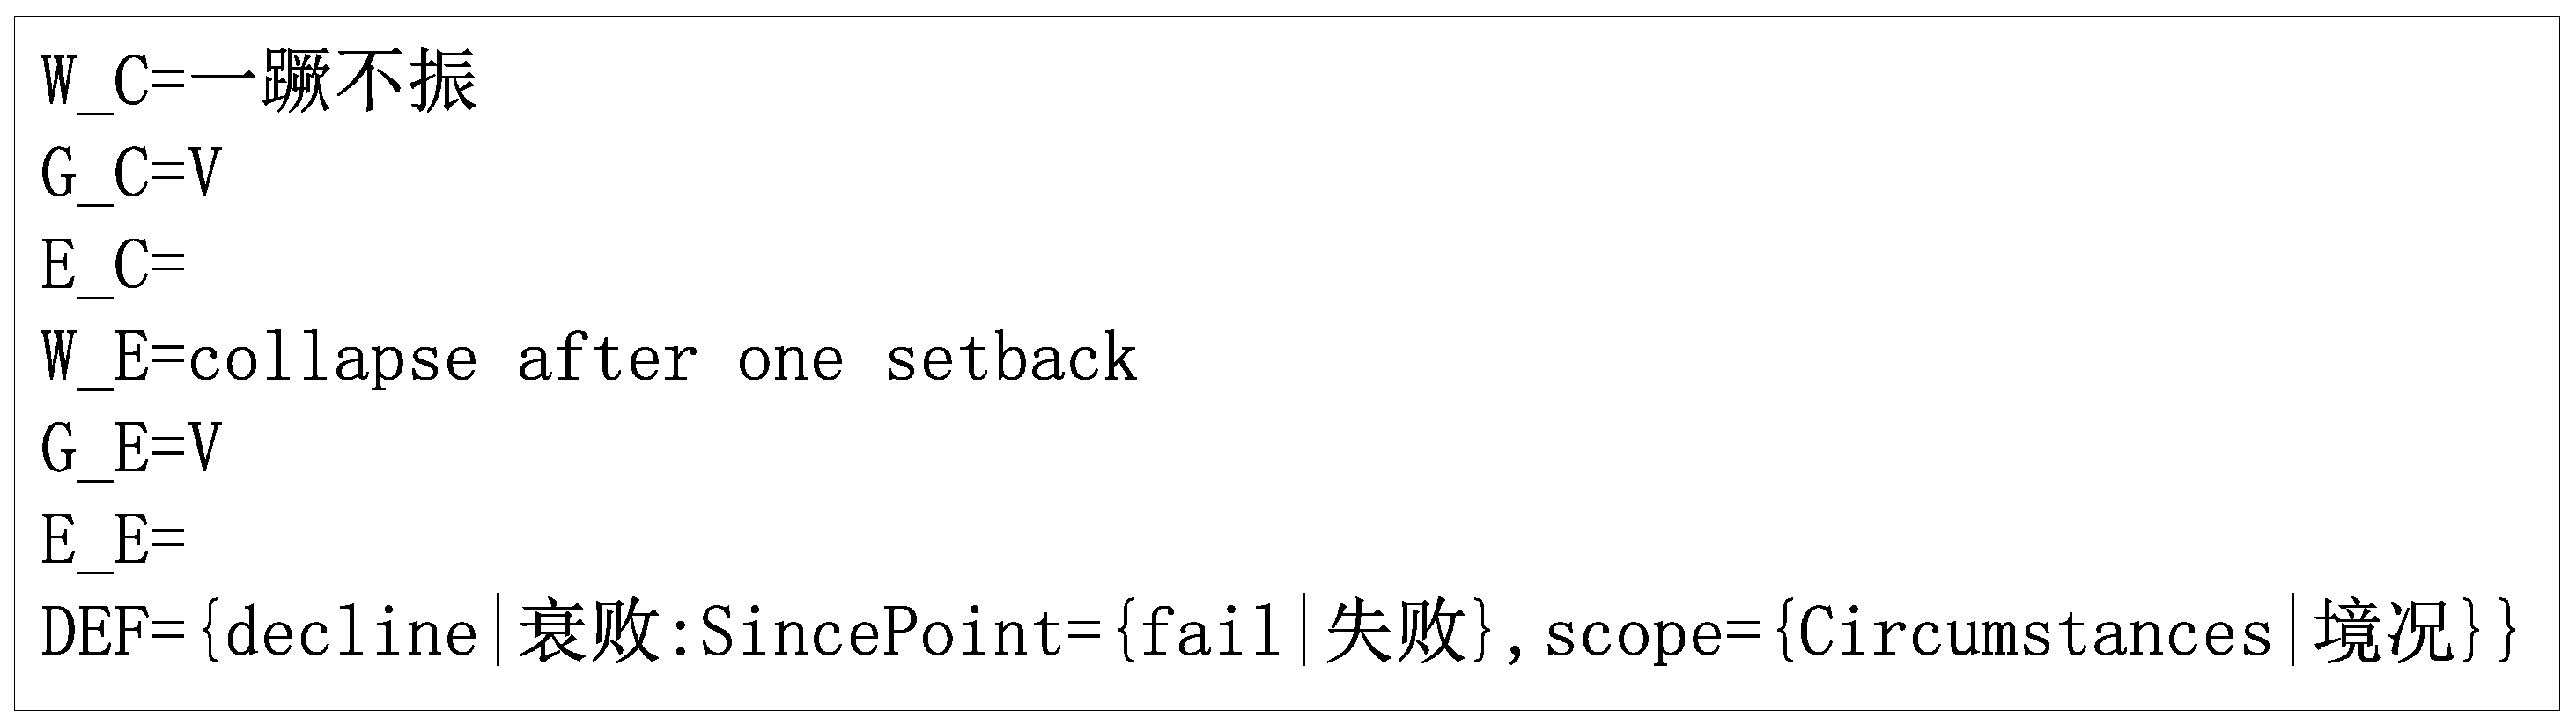
\includegraphics[height=100pt]{2-1-2.eps}
\caption{HowNet中概念描述方式}
\label{fig2-3}
\end{figure}
DEF是HowNet对于概念的定义,称为语义表达式,是知网的核心。HowNet知识描述语言是比较复杂的,为了后续分析计算,我们归纳为以下几条:
\begin{enumerate}
\item HowNet收录词语主有两类,即实词和虚词;
\item 虚词描述比较简单,用“\{句法义原\}”或“\{关系义原\}”进行描述,虚词不具情感极性;
\item 实词的描述就比较复杂了,由一系列用逗号隔开的语义描述式组成,其中语义描述式分为三种形式:
     \begin{enumerate}
     \item 独立义原描述式:用“基本义原”,或“(具体词)”描述;
     \item 关系义原描述式:用“关系义原=基本义原”,或“关系义原=(具体词)”,或“(关系义原=具体词)”描述;
     \item 符号义原描述式:用“关系符号 基本义原”或者“关系符号(具体词)”加以描述;
     \end{enumerate}
\item 实词描述代表了该词的语义知识,因为实词一般具有语义倾向性(如果将中性也视为倾向性的话),因此实词的描述式可以帮助我们确定语义倾向性。
\end{enumerate}

\subsection{WordNet语义词典}
WordNet是由Princeton大学的心理学家、语言学家和计算机工程师联合设计的一种基于认知语言学的英文词典\upcite{Fellbaum1998}。WordNet是根据词义而不是词形来组织词汇信息。如图~\ref{fig2-2-3}所示,WordNet使用同义词集合(Synset)代表概念,词汇关系在词语之间体现,语义关系在概念之间体现。WordNet将英语的名词、动词、形容词和副词组织为Synsets,每一个Synset表示一个基本的词汇概念,并在这些概念之间建立了包括同义关系(synonymy)、反义关系(antonymy)等多种语义关系。其中,WordNet最重要的关系就是词的同义反义关系。

\begin{figure}[htp]
\centering
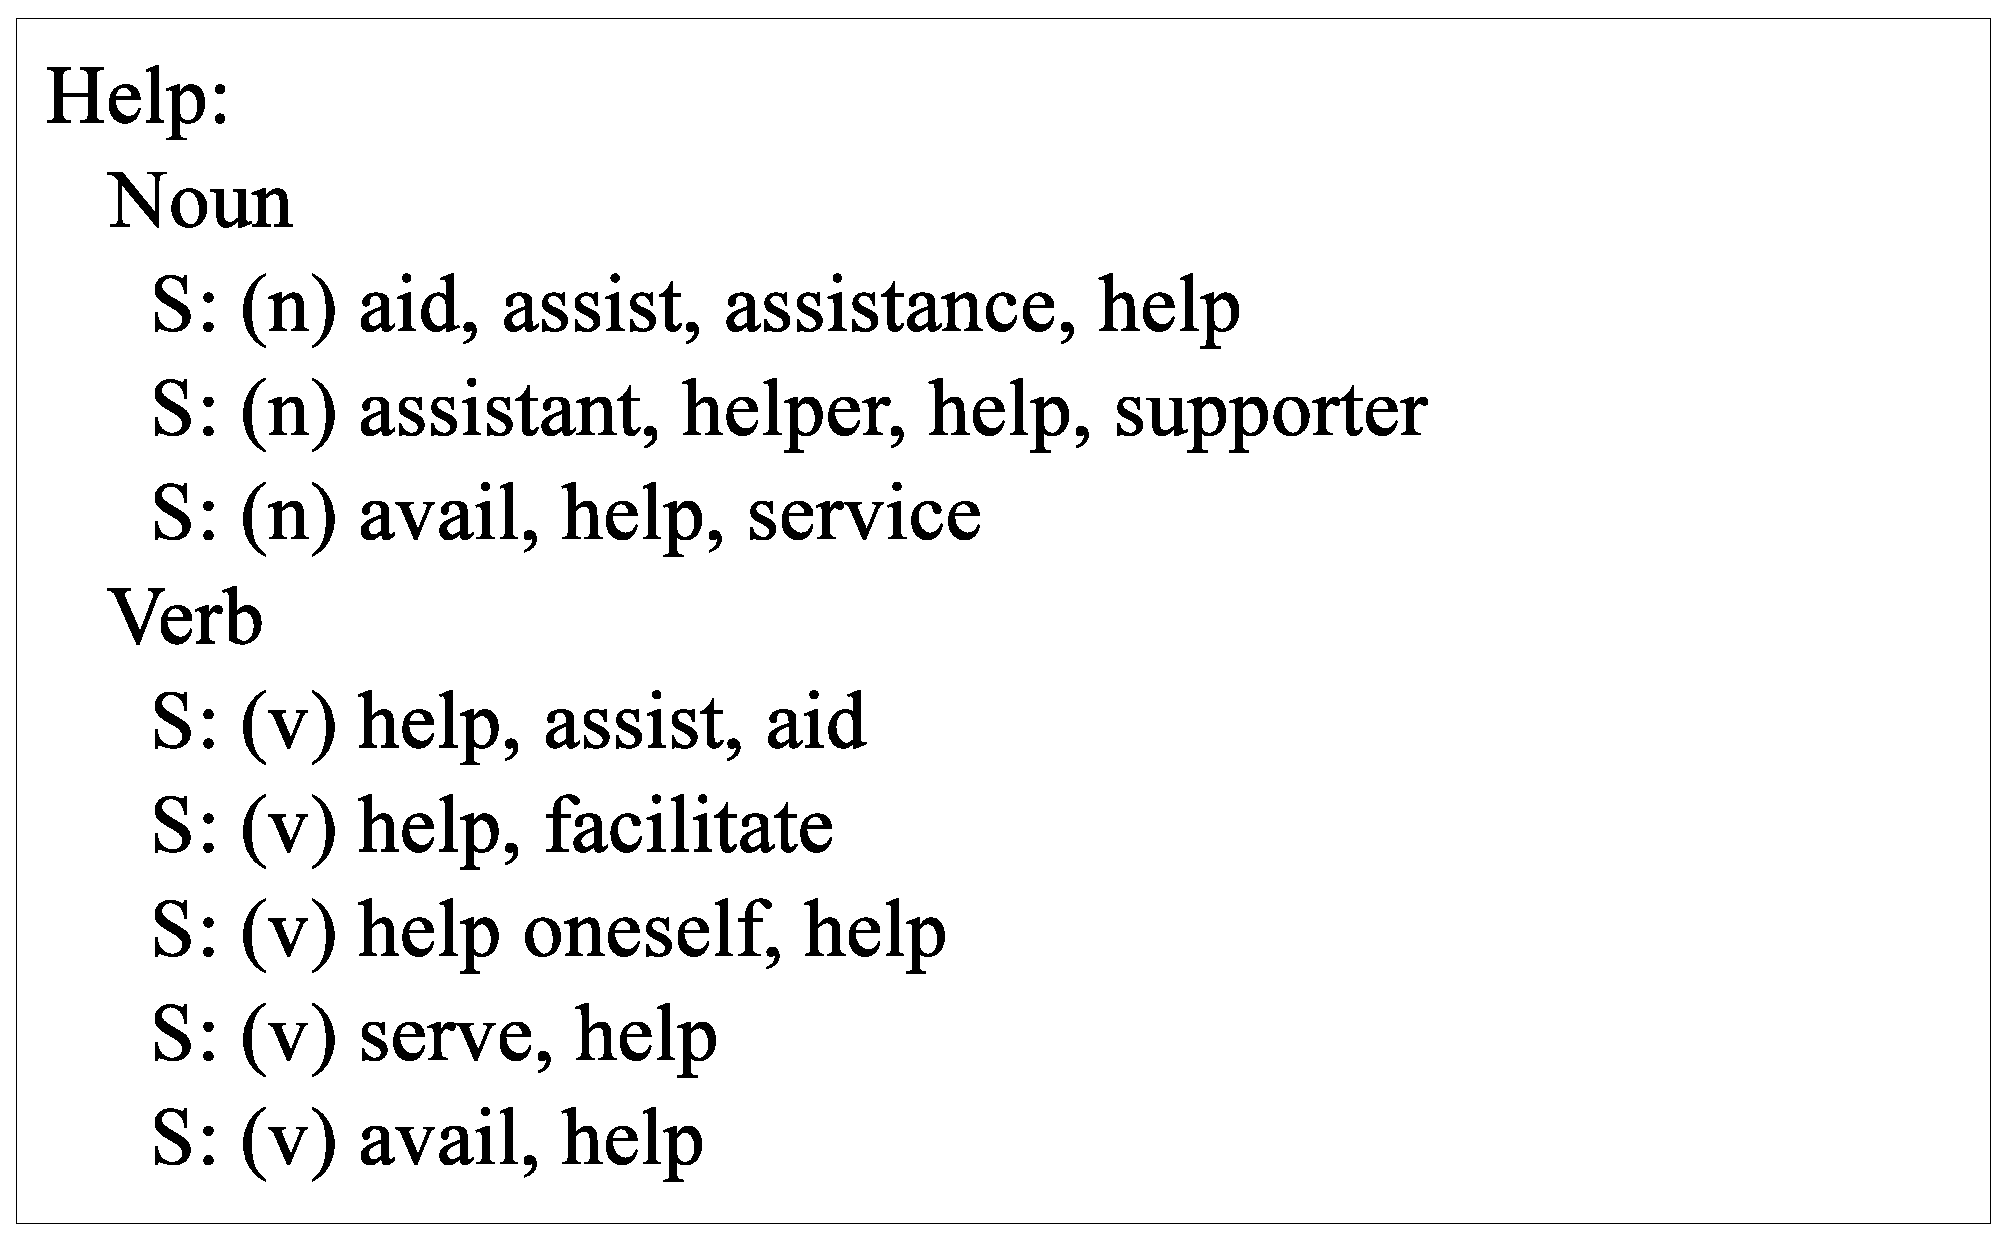
\includegraphics[height=180pt]{2-1-3.eps}
\caption{WordNet单词描述方式}
\label{fig2-2-3}
\end{figure}

\subsection{SentimentWordNet情感词典}
SentimentWordNet是Baccianella\upcite{Baccianella2010}等在语义词典WordNet基础上使用随机游走的图算法计算得到的情感词典。如图~\ref{fig2-2-4}所示,SentimentWordNet的每条记录都是一个WordNet的Synset条目,并且每个Synset都计算出了褒义、贬义情感极性的强度值(简称情感极性值),本章就是利用SentimentWordNet的情感极性值以及HowNet概念的语义关系进行计算得到中文词语的情感极性值,实现从英文情感词典到中文情感词典的情感知识转化。SentimentWordNet共有收录了117,000多个Synsets,约192,493单词。

\begin{figure}[htp]
\centering
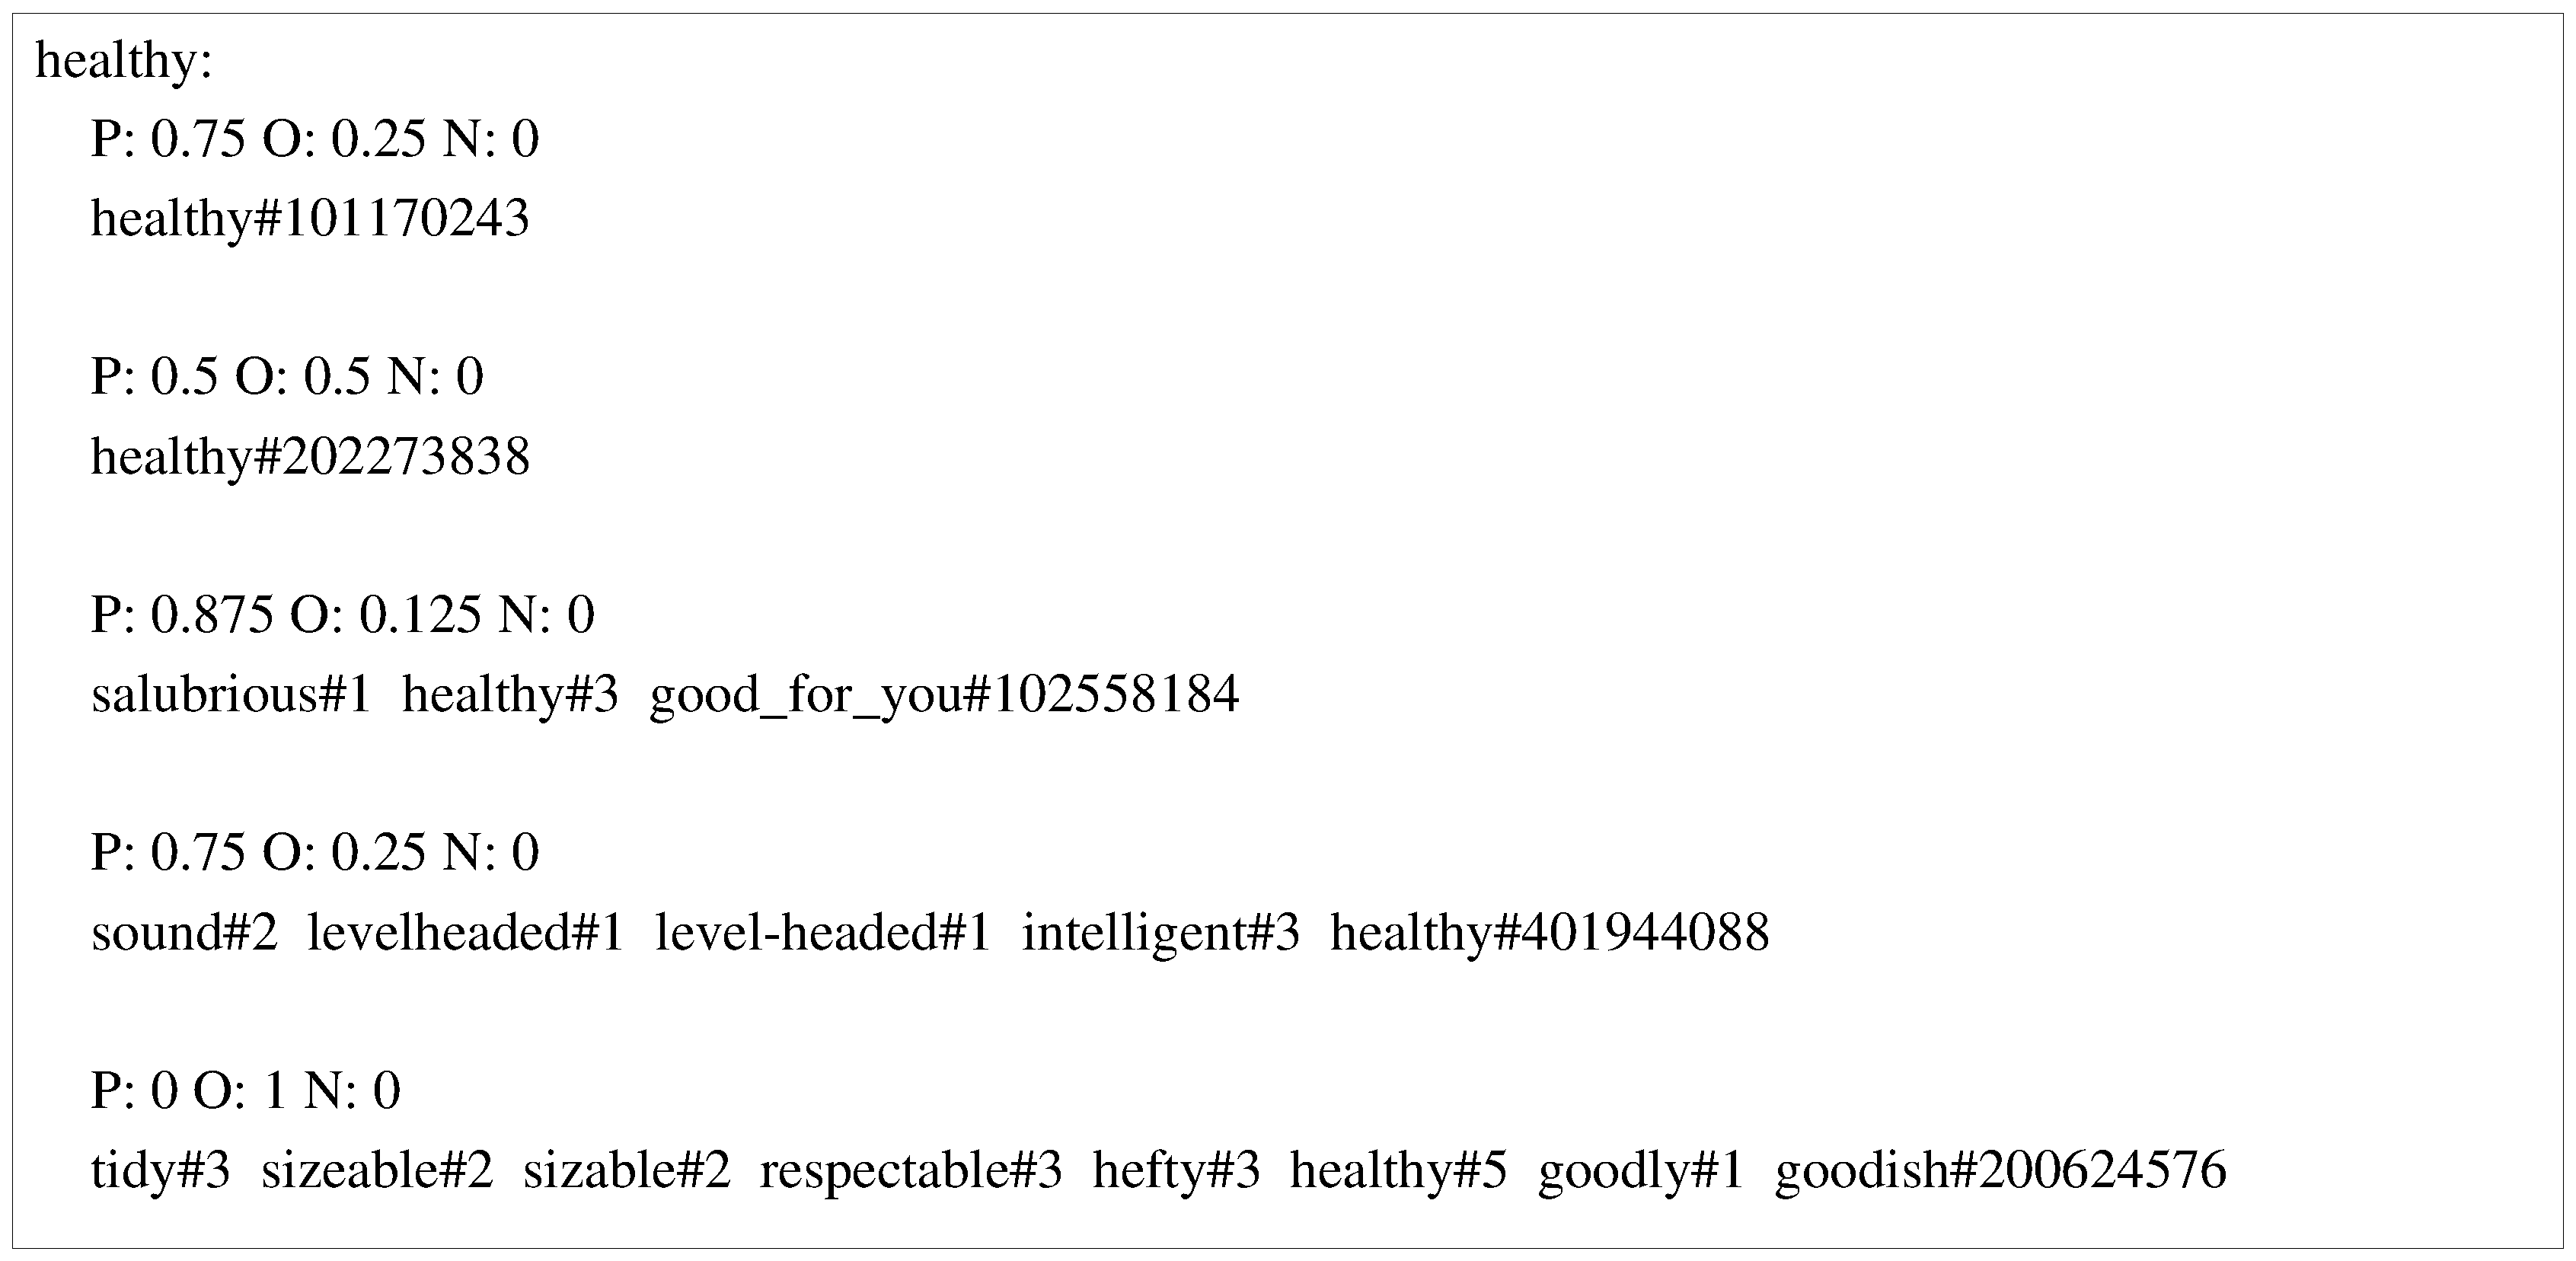
\includegraphics[height=220pt]{2-1-4.eps}
\caption{SentimentWordNet情感词描述方式}
\label{fig2-2-4}
\end{figure}

\section{基于语义关系的情感词典构建方法}
如本章相关工作部分所述,要构建一个新的情感词典有两种方式,一是从头开始(from scratch),另外一种就是通过转化(adaption)其他词典资源的方式。中文观点分析的研究在最近几年才开始受到重视,并且主要是借鉴英文研究已有的资源和方法。中文和英文语法结构和语义表示上存在很大的差别,直接套用英文的资源和研究方法会出现“水土不服”,比如直接将英文情感词典通过翻译方式转化的中文情感词典,是一个从英文情感知识到中文情感知识“给”的方式转化,是将英文情感词典内容映射到中文情感词典,因此存在歧义较大,覆盖度较低以及可靠性不高等问题,并且词典中不可避免存在翻译带来的错误。
本章我们提出一个从中文到英文情感词典去“取”的方式转化情感知识,是从中文情感词典内容到英文情感词典的逆映射,因此可以根据中文词语的语义单元选择英文对应语义单元然后转化情感知识,有效避免了歧义,而且不受覆盖度的限制,可靠性也更高。
同时可以直接将英文中对情感极性值的计算结果直接转化为中文词语的情感极性值,减少了计算开销。本章研究正是基于这种动机展开的,提出的解决方案如图~\ref{frame}框架所示。

具体来说,我们使用了双语语义知识库HowNet作为我们中文词语的来源以及对应英文查询词语的来源。HowNet对义原和概念(大部分都有英文标注)进行了英汉双语标注,可以作为中英文情感知识转化的“桥梁”。我们的计算框架中,每个词语的情感极性值的计算都是由三部分组成,首先是词语对应的英文标注可以从英文情感词典中查询获得情感极性值,第二部分是词语的语义描述DEF中会有义原的英文标注,也可以查询得到情感极性值,第三部分通过对语义描述DEF的语义关系分析,按照义原在DEF中的语义角色对其情感极性值加权后与第一部分进行组合计算词语的最终情感极性值。

HowNet中词语本身有些没有英文标注,无法通过查询英文情感词典获得情感极性值。有些词语虽然有英文的标注,但是查询英文情感词典时候会遇到一词多义问题,不同语义对应的情感极性值不尽相同,得到的情感极性值也会因为存在歧义而不准确。还有一些词语标注的英文是多个单词,无法直接得到情感极性值。HowNet中词语的语义由概念表示,每个概念都有对应的语义描述DEF,DEF是由一个到多个义原按语义关系组合在一起的,因此概念在中文中是没有歧义的。我们正是利用了HowNet中概念语义描述部分,分析其中义原以及义原之间的关系,将义原情感极性值组合计算出词语的情感极性值。HowNet中义原是描述语义最基本的单位,因此我们假设义原的情感极性是确定的,因此通过语义关系组合计算出的情感极性值也应该是确定的,因此可以词语的情感极性进行“消歧”。

综上所述,本章构建情感词典需要解决的问题描述如下:
\begin{enumerate}
\item 如何基于英文情感词典计算义原的情感极性值?
\item 如何通过概念描述中的语义关系分析组合计算概念的情感极性值?
\item 最后如何确定词语的情感极性值?
\end{enumerate}

针对这的三个问题,我们通过情感词语及义原抽取、义原情感极性值计算、以及词语情感极性值计算三个部分进行阐述。

\begin{landscape}
\begin{figure*}
\centering
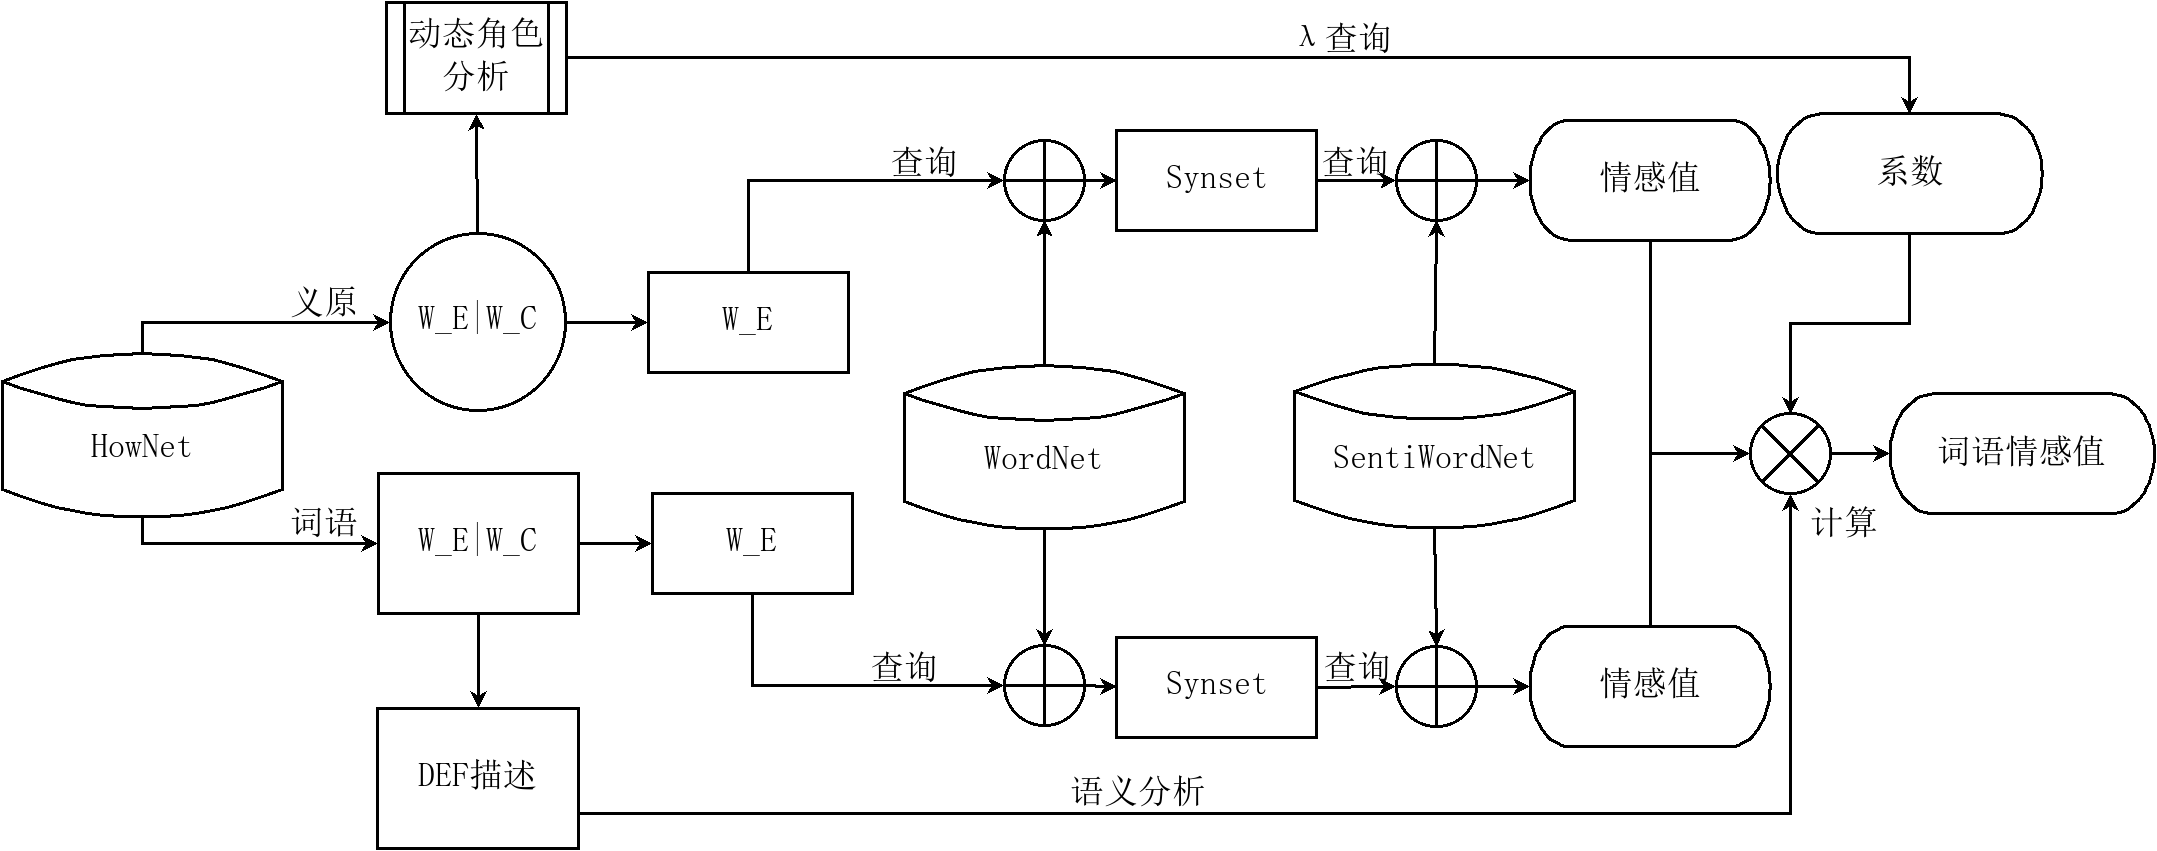
\includegraphics[height=280pt]{2-2.png}
\caption{基于语义关系的情感词典解决方案}
\label{frame}
\end{figure*}
\end{landscape}

\subsection{词语和义原抽取}
词语抽取主要是从HowNet中抽取词语(W\_C)和概念描述(DEF),并对DEF进行分析得出其组成义原及语义关系描述符。在进行词语情感极性值计算时,需要根据DEF中义原和语义关系描述符进行词语的语义分析和极性值计算。情感词语和义原抽取处理流程如图~\ref{atom}所示。

\begin{figure}[htp]
\centering
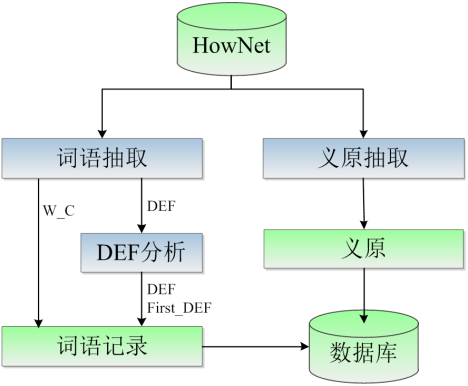
\includegraphics[height=170pt]{2-3.png}
\caption{词语和义原抽取处理流程}
\label{atom}
\end{figure}

从HowNet中抽取出的词语,定义其记录格式如图~\ref{fig2-2-1}所示。
在抽取得到的词语记录中,主要关注的内容有词语编号(No\.)、中文词语(W\_C)、中文词性(G\_C)、英文词语(W\_E)、英文词性(G\_E)、属性(DEF)、第一属性(First\_DEF)等。其中第一属性是指位于属性DEF第一位置的义原,通过第一属性可以分析出该词语所属的特征类。

\begin{figure}[htp]
\centering
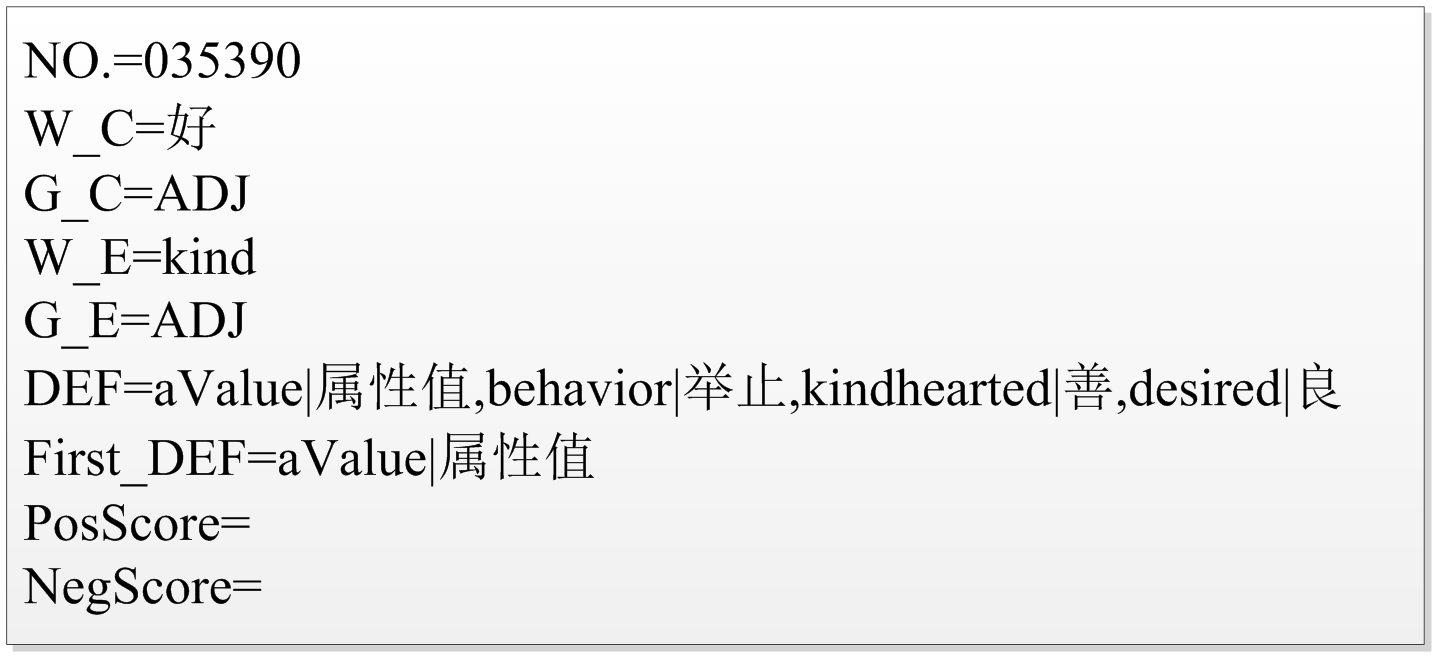
\includegraphics[height=125pt]{2-2-1.png}
\caption{抽取词语记录格式}
\label{fig2-2-1}
\end{figure}

从HowNet中抽取得到的义原的记录格式如图~\ref{fig2-2-2}所示。在抽取得到的义原的记录中,主要关注的内容有词语编号(No\.)、特征类别(Category)、中文词语(W\_C)、英文词语(W\_E)、属性(DEF)、层次(Layer)、父亲节点编号(Father)等。根据记录中的层次(Layer)和父亲节点编号(Father)可以得到义原之间的层次关系,如编号为33的义原“依靠”位于“事件类(Event)”的第五层,其父亲节点编号为32,通过查询编号为32的义原,得到其父亲节点义原为“有关(relate)”。

\begin{figure}[htp]
\centering
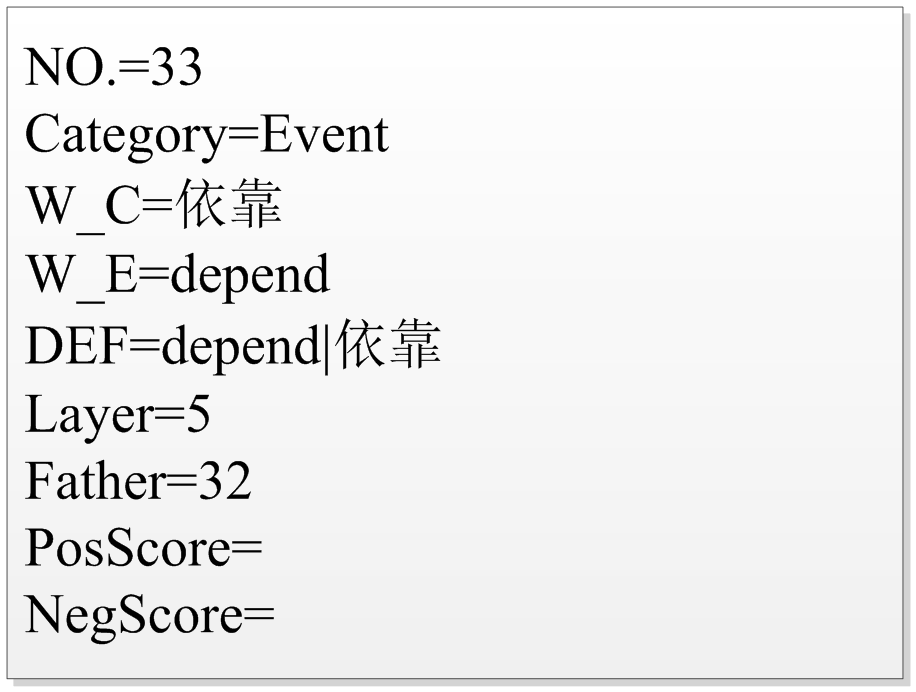
\includegraphics[height=125pt]{2-2-2.png}
\caption{抽取义原记录格式}
\label{fig2-2-2}
\end{figure}

\subsection{义原情感极性值}
这三个部分中义原的情感极性值的确定是非常关键的,是计算词语情感极性值的基础。在HowNet中义原都使用中英双语标注,基本都可以根据英文标注查询得到情感极性值(称为查询类义原极性值)。也有一部分义原英文标注由多个单词连接组成(如“FreeOfCharge$ | $免费”),无法直接查询得到情感极性值,可以通过在上下位关系树中与其他义原的语义距离进行计算获得(称为计算类义原极性值)。最后可以通过义原间的反义和对义关系对计算出的义原情感极性值进行校正。

\subsubsection{查询类义原极性值}
WordNet是以词义(Sense)来记录的,Sense以同一词义的词集Synset表示。通过查询可以得到词语W\_E所有的Sense,将每个Sense映射到SentimentWordNet就可以得到对应的情感极性值。
基于WordNet和SentimentWordNet的义原极性值计算过程如图~\ref{atomsen}所示。

\begin{figure}[htp]
\centering
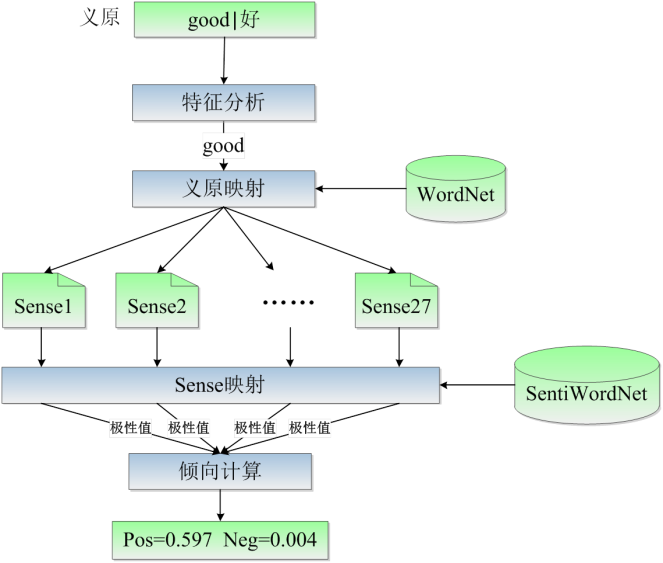
\includegraphics[height=250pt]{2-4.png}
\caption{义原情感极性值计算过程}
\label{atomsen}
\end{figure}

在HowNet中获取义原后将义原对应英文单词(如“good”)映射到WordNet中进行查询,得到该词语所有的Sense(如“good”的Sense共有27个);将这些Sense再映射到SentimentWordNet中查询得到对应Sense情感极性值;将情感极性值加权根据公式~\ref{eq1}计算得到义原的情感极性值(如“good”的极性值为PosScore=0.597,NegScore=0.004)。
\begin{equation}
\label{eq1}
\varphi(s,p)=\dfrac{\sum_{i=1} \varphi_i (s,p)}{\sum_{p\in P}\sum_{i=1}^m \varphi_i(s,p)}
\end{equation}

公式中$ P$表示极性类型(积极、消极、中性,“P、N、O”),$m$为与义原相对应的Sense的总数,$s$表示义原,$\varphi(s,p)$表示义原的极性值,$\varphi_i (s,p)$表示义原在编号为$ i $的Sense中的$ p $类型极性值。

\subsubsection{计算类义原极性值}
经过上面的查询计算过程,可以得到大部分义原的情感极性值。由于所有的义原根据上下位关系构成了一个树状的义原层次体系,针对一些无法查询计算得到的义原,我们采用简单的通过语义距离计算相似度的办法间接计算出情感极性值。假设两个义原(一个情感极性值已知,一个未知)在层次体系中的路径距离为$ d $,根据公式~\ref{eq2-1},我们可以得到这两个义原之间的语义距离:
\begin{equation}
\label{eq2-1}
sim(s_i,s)=\dfrac{\alpha}{d+\alpha}
\end{equation}
其中$ s_i $是情感极性值已知义原,$ s $表示需要情感极性值计算的义原,$ d $是$ s_i $和$ s $在义原层次体系树中的路径长度。$ \alpha $是一个可调节的参数,一般$ \alpha=0.5 $。

为了能够在上位和下位义原的情感极性值取得平衡,对任意一个情感极性值未知义原$ s $,都要计算$ s $与最靠近$ s $极性值已知的上位义原$ s_1 $ 和下位义原 $ s_2 $之间的语义距离:$sim(s_1,s)$和$sim(s_2,s)$。然后从上位义原$ s_1 $ 和下位义原 $ s_2 $的情感极性值加权平均得到$ s $的情感极性值。
\begin{equation}
\varphi(s,p)=sim(s_1,s)\varphi(s_1,p)+sim(s_2,s)\varphi(s_2,p)
\end{equation}

\subsubsection{情感极性值校正}
所有义原在前面两种方法计算得到情感极性值会存在一些偏差(bias),有些义原偏差会比较大,甚至计算得到的极性值与义原的真实语义倾向相反(如“FreeOfCharge$ | $免费”义原计算得到极性值为PosScore=0.07,NegScore=0.236),因此需要通过利用HowNet中的其他语义关系对上述计算方法进行校正。我们采用了基于HowNet中对义和反义语义关系进行义原情感极性值校正。对于任一义原$ s $,对义或反义义原为$ \overline{s} $,对$ s $情感极性值修正为:
\begin{equation}
\varphi(s,p)=\dfrac{|\varphi(s,p)-\varphi(\overline{s} ,p)|}{2}
\end{equation}



\subsection{词语情感极性值}
词语情感值可以通过两种途径获得,一是通过词语本身的英文标注直接查询英文情感词典,这种方式并不可靠而且存有歧义;二是根据词语的语义描述DEF中的义原的情感极性值计算得出,这种方式相对可靠,每个义原都有确定的情感极性值,因而不存在歧义。为了计算词语的情感极性值,需要对语义描述DEF中的语义关系进行分析,因为义原间的语义关系会引起义原情感值的反转以及在描述语义倾向时的权重变化。
因此首先对HowNet中因为DEF的语义关系不同引起的情感极性值变化提出如下定义:
\begin{definition}[情感极性值反转]
义原$s$的$p$极性值$\varphi(s,p)$取反运算是,将$s$的积极极性值和消极极性值互换,过程如公式~\ref{2-2}:
\begin{equation}
\label{2-2}
\overline{\varphi(s,p)}=\varphi(s,q),\quad (p,q) \in P\&\& p \neq q
\end{equation}
\end{definition}
事件类义原有很多在DEF描述中可以引起情感极性值的变化,比如“DoNot$ | $不做,lose$ | $失去”等相当于句子中的否定词,会引起其他词语情感极性值反转,因此我们从819个事件类义原中挑选了在语义描述中起否定作用的义原称为极性反转语义角色,并加以标记。
\begin{definition}[情感极性值加权]
 $\lambda$因子与义原$s$的$p$极性值的加权运算定义为$\lambda$乘法运算,过程如公式~\ref{2-3}:
\begin{equation}
\label{2-3}
\lambda \times \varphi(s,p) =\begin{cases}
& \lambda \varphi(s,p), \quad  \lambda >0\\
& 0, \quad\quad  \lambda=0\\
&|\lambda|\varphi(s,p), \quad  \lambda <0
\end{cases}
\end{equation}
\end{definition}

公式~\ref{2-3}中$\lambda$取值范围为$ (-1,0,1) $,具体值需要根据关系义原描述式中的关系义原(动态角色义原)和符号义原描述式中的符号义原确定。符号义原中只有“$ \wedge$”(表示“非”的关系)会改变语义倾向,因此“$ \wedge$”所修饰的义原在计算中权重为$\lambda=-1$。
HowNet中共有90个动态角色义原,我们分别对每个义原进行了分析,确认了其语义关系角色所确定的基本义原的权重取值$\lambda$。
如词语“扭亏为盈”的DEF描述为“DEF=alter|改变,StateIni=InDebt|亏损,StateFin=earn|赚”,义原“InDebte|亏损”为初始状态(StateIni),“earn|赚”为最终状态(StateFin),经过分析后,StateIni描述的“InDebte|亏损”的$\lambda$取值为0,StateFin描述的“earn|赚”的$\lambda$取值为1。

最后词语的情感极性值计算总结为公式~\ref{2-4}。其中$\varphi(w,p)$表示词语$w$的$p$极性值,$s_i$表示词语DEF中第$i$个义原,$n$为词语DEF中义原总数。
\begin{equation}
\label{2-4}
\varphi(w,p)=\dfrac{\sum_{i=1}^n\lambda_i\times\varphi(s_i,p)}{\sum_{p\in P}\sum_{i=1}^n\lambda_i\times\varphi(s_i,p)}
\end{equation}
其中:$\sum_{p \in P}\varphi(w,p)=1$。

对于已经通过查询得到情感极性值的词语(有多个英文Sense对应的词语的情感极性值$\varphi(\overline{w},p)$可以取所有Sense对应极性值的加和平均),可以和通过语义描述DEF计算得到的极性值加权累加,计算公式为:
\begin{equation}
\Psi(w,p)=\alpha \varphi(w,p)+(1-\alpha)\varphi(\overline{w},p)
\end{equation}
其中$ \alpha \in (0,1)$的取值要考虑那种方式得到的情感极性值更准确,一般将$ \alpha $取偏大些以反映语义描述DEF对词语语义倾向性的影响更大。

\section{实验}
情感词典的实验评测有两种方法,一是直接评测,将情感词典与人工编辑的或者其他可靠性较高的词典进行对比评测;二是间接评测,将情感词典应用到文本情感分类任务评测其性能。本节我们使用直接评测的方法。

\subsection{直接评测}
在实验评测时,采用HowNet评价词词典基准。HowNet评价词词典是2007年发布的人工标注的词典,每个词语只标注积极和消极极性,没有极性值。HowNet评价词词典中情感词共有6497项,其中积极极性词语3436项,消极极性词语3061项。

我们将本章中利用HowNet中的语义关系构建的情感词典命名为SentiHowNet。SentiHowNet的词语都有积极极性值和消极极性值,为了和HowNet评价词词典作对比评测,按照公式~\ref{eq2-5}对SentiHowNet的每个词计算得出一个极性。
\begin{equation}
\label{eq2-5}
\begin{cases}
positive \qquad & score(w)>T\\
negative \qquad & score(w)<-T
\end{cases}
\end{equation}
其中$ score(w)= \varphi(w,P)-\varphi(w,N)$为词语$ w $积极极性值与消极极性值相减得到的差值,$ T $为阈值,差值$ score(w)$高于$ T $则词语$ w $情感极性为积极极性,差值$ score(w)$低于$ -T $则词语$ w $情感极性为消极极性。当$ T=0 $时,我们构建的SentiHowNet有积极极性情感词12433项,消极极性情感词11148,词典的整体规模达到23581个条目。

评价指标采用常用的精准率(P)、召回率(R)以及F值。
\subsubsection{阈值T的设定}
首先考察不同的阈值$ T $对词典评价指标的影响,以确定一个合理的阈值。
图\ref{fig2-5}为$ T $的不同取值对词典性能指标的影响,实验中我们将$ T $的值由0逐渐增加,当$ T $大于0.1时性能指标基本没有变化或成下降趋势。从图中可以看出,在$ T=0 $时,虽然召回率最高达到88.58\%,但精准率最低仅有54.40\%,F值仅为67.40\%。当$ T=0.05 $时,精准率提高到77.75\%,有较大提高,召回率仅下降到87.61\%,下降幅度较小,F值提高到82.39\%。当$ T $提高到0.05时性能指标达到最好,因此可以设定$ T $为0.05。

\begin{figure}[htp]
\centering
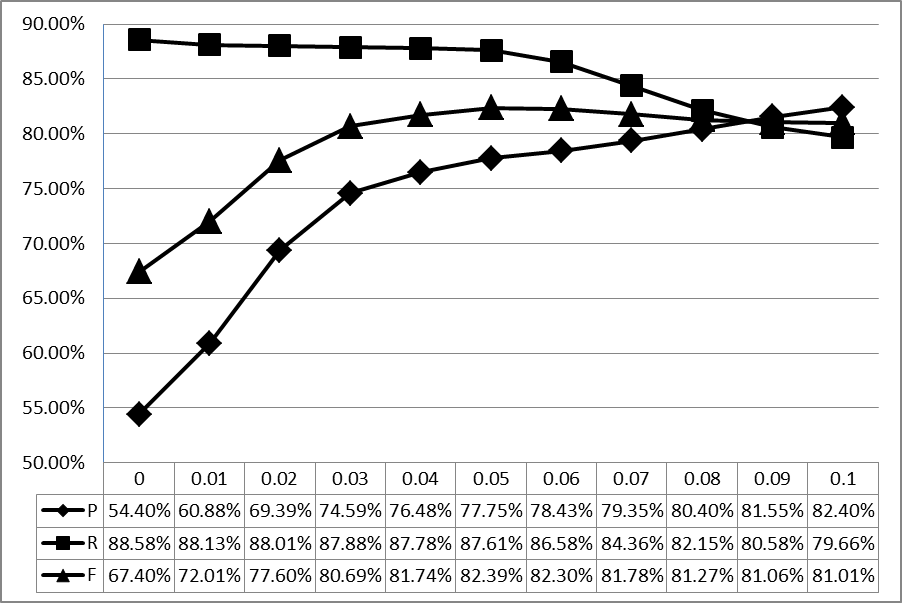
\includegraphics[height=250pt]{2-5.png}
\caption{不同T值时的性能指标}
\label{fig2-5}
\end{figure}

\subsubsection{与其他词典性能对比}
确定了阈值T以后,我们将SentiHowNet与目前常用的中文情感词典NTUSD词典(11086个中文词汇,2810积极极性词语,8276消极性词语)\upcite{Ku2007}以及大连理工大学的情感词汇本体词库(用DLLEX标记,17156条目,10627个积极极性词语,6529个消极极性词语)\upcite{徐琳宏2008}进行对比评测,首先是三个词典对评价基准词典的覆盖度对比,结果如表~\ref{tab2-2}所示。从表中可以看出,按照积极和消极极性分来来看,在积极极性词中SentiHowNet词典覆盖度最好,NTUSD词典由于包含的积极极性词数量少因此覆盖读最低;在消极极性词中,NTUSD词典的覆盖度最好,SentiHownet和DLLEX词典覆盖度基本一样。四种个词典中除了作为基准词典的HowNet评价词词典,采用我们设计方法在HowNet上自动构建的情感词典SentiHowNet包含情感词条目(注意经过阈值T=0.05过滤后)最少,但是对基准词典的覆盖度最高(总体准确标注数达到6092),主要原因是SentiHowNet本身就是从HowNet自动产生,是HowNet包含词语的子集,而NTUSD和DLLEX词典中词语的来源不同,因此会有覆盖度的偏置。

\begin{table}[htp]
\centering
\caption{词典覆盖度}
\label{tab2-2}
\begin{tabular}{|l|l|l|l|l|l|l|}
\hline
\multicolumn{1}{|c|}{\multirow{2}{*}{词典}} & \multicolumn{2}{c|}{积极极性} & \multicolumn{2}{c|}{消极极性} & \multicolumn{2}{c|}{总体统计} \\ \cline{2-7} 
\multicolumn{1}{|c|}{} & \multicolumn{1}{c|}{标注} & \multicolumn{1}{c|}{正确} & \multicolumn{1}{c|}{标注} & \multicolumn{1}{c|}{正确} & \multicolumn{1}{c|}{标注} & \multicolumn{1}{c|}{准确} \\ \hline
HowNet & \multicolumn{2}{c|}{3436} & \multicolumn{2}{c|}{3061} & \multicolumn{2}{c|}{6497} \\ \hline
NTUSD & 2810 & 2204 & 8276 & 3022 & 11086 & 5226 \\ \hline
DLLEX & 10627 & 3020 & 6529 & 2876 & 17156 & 5896 \\ \hline
SentiHownet & 4256 & 3218 & 5113 & 2874 & 9369 & 6092 \\ \hline
\end{tabular}
\end{table}

在T=0.05时,SentiHowNet与其他词典性能比较如表~\ref{tab2-3}所示。在积极极性词语的性能对比中,SentiHowNet词典的精确率和F值最好,分别达到了93.66\%和83.67\%,但是召回率(75.\%61)比NTUSD词典(78.43\%)略差;在消极极性词语的性能对比中,三个词典的精确率都比较高(都超过90\%),但是召回率比较低,NTUSD词典精确率最好,达到98.\%73,而SentiHowNet词典在召回率和F值上性能最好;总体来看,宏平均指标中SentiHowNet词典精准率为93.77\%,召回率为65.02\%,F值为76.79\%,均为三个词典中最高。
\begin{table}[htp]
\centering
\caption{词典性能对比}
\label{tab2-3}
\begin{tabular}{|l|c|c|c|c|c|c|c|c|c|}
\hline
\multicolumn{1}{|c|}{\multirow{2}{*}{词典}} & \multicolumn{3}{c|}{积极极性} & \multicolumn{3}{c|}{消极极性} & \multicolumn{3}{c|}{宏平均} \\ \cline{2-10} 
\multicolumn{1}{|c|}{} & P & R & F & P & R & F & P & R & F \\ \hline
NTUSD & 0.6414 & \textbf{0.7843} & 0.7057 & \textbf{0.9873} & 0.3652 & 0.5331 & 0.8044 & 0.4714 & 0.5944 \\ \hline
DLLEX & 0.8789 & 0.2842 & 0.4295 & 0.9396 & 0.4405 & 0.5998 & 0.9075 & 0.3437 & 0.4985 \\ \hline
SentiHownet & \textbf{0.9366} & 0.7561 & \textbf{0.8367} & 0.9389 & \textbf{0.5621} & \textbf{0.7032} & \textbf{0.9377} & \textbf{0.6502} & \textbf{0.7679} \\ \hline
\end{tabular}
\end{table}

以上两个对比表明相对于需要人工干预的人工或半自动方法构建的情感词典,使用我们设计的自动构建情感词典方法可以构建一部覆盖度比较好,性能又可靠的情感词典,同时节省了不必要的人力开销。

\section{小结}
本章对中文情感词典构建相关研究进行了分类和详细阐述,基于目前中文情感词典研究现状,提出了一种新的词典跨语言自动转化方法。该方法以双语语义知识库HowNet、WordNet语义词典和SentimentWordNet情感词典为基础,根据HowNet对词语语义定义和描述的特点,通过双语标注将HowNet义原和词语情感值转换为英文情感词典对应词语的查询与计算。具体来说,中文词语的情感极性值计算被分解为三个部分,分别为义原情感值的计算与校正,词语语义描述的语义关系分析以及最终的词语情感值的计算。按照该方法最终形成情感词典SentiHowNet,词典的规模为:有积极极性情感词12433项,消极极性情感词11148,词典的整体规模达到23581个条目。在实验部分,采用了直接评测的方法,以人工编辑的HowNet评价词典为基准,在覆盖度、精确率、召回率以及F值等指标上与现有的常用情感词典NTUSD和DLLEX词典进行了实验对比。实验结果表明,SentiHowNet对基准词典的覆盖度最好,宏平均的精确率、召回率以及F值最高,证明了该自动构建情感词典方法的有效性,避免了人工和半自动方法的人工干预开销。